\documentclass[17pt]{extarticle}
\usepackage{fontspec}
\usepackage{geometry}
\geometry{a4paper, margin=2.1cm}
\usepackage{graphicx}
\usepackage{booktabs}
\usepackage{array}
\usepackage{amsmath}
\usepackage{amssymb}
\usepackage[table]{xcolor}
\usepackage{titlesec}
\usepackage{fancyhdr}
\renewcommand{\contentsname}{\color{theme}สารบัญ}
\usepackage{enumitem}
\usepackage[most]{tcolorbox}
\usepackage{hyperref}

\definecolor{theme}{HTML}{2b6a77}
\definecolor{themeD}{HTML}{1f4e58}
\definecolor{ink}{HTML}{232d33}
\definecolor{ok}{HTML}{3f8161}
\definecolor{warn}{HTML}{b5651d}
\definecolor{cardbg}{HTML}{f3f6f7}
\definecolor{softgray}{HTML}{eef1f2}
\definecolor{exbg}{HTML}{eef4f0}
\hypersetup{colorlinks=true, linkcolor=theme, urlcolor=theme, pdftitle={Report For Noob - SPR Fracture Detection}}

\setmainfont{THSarabunNew.ttf}[
  Path=./fonts/, BoldFont=THSarabunNew Bold.ttf,
  ItalicFont=THSarabunNew Italic.ttf, BoldItalicFont=THSarabunNew BoldItalic.ttf]
\setmonofont{cour.ttf}[Path=./fonts/, BoldFont=courbd.ttf, Scale=0.80]
\XeTeXlinebreaklocale "th"
\XeTeXlinebreakskip = 0pt plus 0.1pt

\titleformat{\section}{\Large\bfseries\color{theme}}{\thesection.}{0.5em}{}
\titleformat{\subsection}{\large\bfseries\color{ink}}{\thesubsection}{0.5em}{}
\setlist{itemsep=2pt, topsep=3pt}
\pagestyle{fancy}\fancyhf{}
\fancyhead[L]{\small\color{ink} Report for Noob --- SPR Fracture Detection}
\fancyhead[R]{\small\color{ink}\thepage}
\renewcommand{\headrulewidth}{0.4pt}
\renewcommand{\headrule}{\hbox to\headwidth{\color{theme!45}\leaders\hrule height \headrulewidth\hfill}}

% concept box
\newtcolorbox{concept}[1]{colback=cardbg, colframe=theme!55, boxrule=0.8pt, arc=3pt, left=8pt, right=8pt, top=4pt, bottom=5pt,
  title={\bfseries #1}, coltitle=white, colbacktitle=theme, fonttitle=\bfseries}
% example box
\newtcolorbox{example}{colback=exbg, colframe=ok!55, boxrule=0.8pt, arc=3pt, left=8pt, right=8pt, top=3pt, bottom=4pt}
% how-to-read box
\newtcolorbox{howread}{colback=softgray, colframe=warn!55, boxrule=0.8pt, arc=3pt, left=8pt, right=8pt, top=3pt, bottom=4pt}
\newcommand{\ex}{\textcolor{ok}{\textbf{ตัวอย่าง:}}\ }
\newcommand{\rd}{\textcolor{warn}{\textbf{อ่านกราฟ:}}\ }
\newcommand{\code}[1]{{\ttfamily\detokenize{#1}}}
\newcommand{\thd}[1]{\cellcolor{theme}\color{white}\textbf{#1}}
\newcommand{\rtab}{\smallskip\par\textcolor{theme}{\textbf{ตารางผล:}}\par\nopagebreak\smallskip}

\begin{document}

\begin{center}
{\color{theme}\rule{\linewidth}{2.5pt}}\\[8pt]
{\Huge\bfseries\color{themeD} Report for Noob}\\[6pt]
{\Large\color{theme} คู่มือเข้าใจง่าย: เราพิสูจน์อะไร และรู้ได้อย่างไร}\\[6pt]
{\large การตรวจจับรอยแตกกระดูกด้วยการกระเจิงรังสีเอกซ์ (SPR)}\\[3pt]
{\small สำหรับผู้อ่านที่\textbf{ไม่คุ้นเคยกับสถิติวิจัย} --- อธิบายทุกอย่างจากศูนย์}\\[3pt]
{\small Baanwit Academy \quad$\bullet$\quad \today}\\[6pt]
{\color{theme}\rule{\linewidth}{2.5pt}}
\end{center}
\vspace{4pt}

\begin{concept}{รายงานนี้คืออะไร?}
เราทำการทดลอง (จำลองด้วยคอมพิวเตอร์) เพื่อตอบคำถามว่า ``รอยแตกกระดูกเล็ก ๆ ทิ้งร่องรอยที่ตรวจจับได้ใน
\textbf{การกระเจิงของรังสีเอกซ์} หรือไม่'' รายงานนี้จะพาคุณไปทีละขั้น: (1)~แต่ละการทดลอง\textbf{ตั้งคำถาม (สมมติฐาน)}
ว่าอย่างไร, (2)~เราใช้\textbf{เครื่องมือสถิติ}อะไรตัดสิน (พร้อมตัวอย่างคำนวณจริง), (3)~\textbf{กราฟอ่านอย่างไร}
และมันบอกอะไร, (4)~สรุปทั้งหมด --- โดย\textbf{ไม่ถือว่าคุณรู้สถิติมาก่อน}
\end{concept}

\vspace{2pt}
{\small\tableofcontents}
\clearpage

% =================================================================
\section{ปูพื้นฐาน: ศัพท์สถิติที่ต้องรู้ (แบบบ้าน ๆ)}
ก่อนดูการทดลอง เรามาทำความรู้จัก ``เครื่องมือ'' ที่ใช้ตัดสินกันก่อน --- อธิบายด้วยภาษาคน

\subsection{สมมติฐาน (Hypothesis) --- คำถามที่จะพิสูจน์}
\begin{concept}{คืออะไร}
\textbf{สมมติฐาน}คือข้อความที่เราจะทดสอบว่าจริงไหม เช่น ``รอยแตกทำให้สัญญาณ SPR เปลี่ยน''. นักสถิติชอบตั้ง
\textbf{คู่ตรงข้าม} 2 อัน: \textbf{H0 (null)} = ``ไม่มีอะไรเกิดขึ้น / เป็นเรื่องบังเอิญ'' และ \textbf{H1} = ``มีผลจริง''.
งานของเราคือหาหลักฐานว่า H0 ไม่น่าจะจริง เพื่อจะเชื่อ H1
\end{concept}

\subsection{ค่าเฉลี่ย, การกระจาย, และ ``สัญญาณเทียบ noise'' (t-value)}
เวลาเราวัดอะไรหลาย ๆ ครั้ง ค่าจะไม่เท่ากันเป๊ะ (มี noise). เราสนใจ 2 อย่าง: \textbf{ค่าเฉลี่ย} (สัญญาณ) และ
\textbf{ความกระจาย} (noise).

\begin{concept}{t-value = สัญญาณหารด้วย noise}
\[ t=\frac{\text{ค่าเฉลี่ย}}{\text{ความคลาดเคลื่อนของค่าเฉลี่ย}}=\frac{\overline{x}}{s/\sqrt{N}} \]
($\overline{x}$ = ค่าเฉลี่ย, $s$ = ส่วนเบี่ยงเบนมาตรฐาน, $N$ = จำนวนครั้งที่วัด). \textbf{$|t|$ ยิ่งมากยิ่งดี} =
สัญญาณเด่นชัดเหนือ noise. โดยคร่าว ๆ $|t|>2$ เริ่มน่าเชื่อ
\end{concept}
\begin{example}
\ex ในการทดลอง CL-0 รอยแตก 0.306~มม.\ เราวัด 8 ครั้ง ได้ค่าเฉลี่ย $\overline{x}=-3.33$ (หน่วย $\times10^{-5}$),
ความกระจาย $s=3.02$. ความคลาดเคลื่อนของค่าเฉลี่ย $=s/\sqrt{8}=3.02/2.83=1.07$. ดังนั้น
$t=-3.33/1.07=\mathbf{-3.12}$ --- แปลว่าสัญญาณ (ค่าเฉลี่ยติดลบ) เด่นกว่า noise ประมาณ 3 เท่า (เครื่องหมายลบ
บอกทิศทาง = SPR ``ลดลง'')
\end{example}

\subsection{p-value --- ``โอกาสที่จะเป็นเรื่องบังเอิญ''}
\begin{concept}{p-value คืออะไร}
สมมติว่า \textbf{จริง ๆ แล้วไม่มีผลอะไรเลย (H0 จริง)} --- \textbf{p-value คือความน่าจะเป็นที่เราจะเห็นผลลัพธ์
สุดขั้วขนาดนี้ (หรือกว่านั้น) โดยบังเอิญ}. \textbf{p น้อย = โอกาสฟลุ๊คน้อย = ผลน่าจะจริง}. เกณฑ์มาตรฐานที่นักวิจัย
ใช้กันคือ \textbf{$p<0.05$} (โอกาสฟลุ๊คต่ำกว่า 5\%) เรียกว่า ``มีนัยสำคัญ (significant)''
\end{concept}
\begin{example}
\ex เปรียบเหมือน\textbf{โยนเหรียญ}: ถ้าเพื่อนบอกว่าเหรียญยุติธรรม (H0) แต่คุณโยนได้หัว 9 ครั้งจาก 10 --- โอกาสที่
เหรียญยุติธรรมจะให้ผลเอียงขนาดนี้โดยบังเอิญมีน้อยมาก (p เล็ก) คุณจึงเริ่มเชื่อว่า ``เหรียญนี้ไม่ยุติธรรม (H1)''.
ในงานเรา CL-0 ที่ 0.306~มม.\ ได้ $p=0.017$ = ถ้ารอยแตกไม่มีผลจริง โอกาสเห็นสัญญาณแรงขนาดนี้โดยบังเอิญ
มีแค่ \textbf{1.7\%} --- น้อยพอจะเชื่อว่าเป็นของจริง
\end{example}

\subsection{ช่วงความเชื่อมั่น (Confidence Interval) และ Bootstrap}
\begin{concept}{95\% CI = ``ช่วงที่ค่าจริงน่าจะอยู่''}
ค่าเฉลี่ยที่เราวัดได้เป็นแค่การประมาณ. \textbf{ช่วงความเชื่อมั่น 95\%} คือช่วงตัวเลขที่เรามั่นใจ 95\% ว่าค่าจริง
อยู่ในนั้น. \textbf{ถ้าช่วงนี้ไม่คร่อมเลข 0} แปลว่าเรามั่นใจว่ามีผลจริง (ไม่ใช่ศูนย์). วิธี \textbf{bootstrap} คือ
เอาข้อมูลที่มีมา ``สุ่มหยิบใหม่ซ้ำ ๆ หลายหมื่นครั้ง'' เพื่อดูว่าคำตอบแกว่งแค่ไหน
\end{concept}
\begin{example}
\ex CL-1 รอยแตก 0.54~มม.: ช่วงความเชื่อมั่น 95\% ของสัญญาณ $=[-6.84,-3.16]$ ($\times10^{-5}$) ---
ทั้งช่วง\textbf{ติดลบหมด ไม่แตะ 0} จึงมั่นใจว่ารอยแตกทำให้ SPR ลดลงจริง
\end{example}

\subsection{การทดสอบด้วยการสลับ (Permutation / Null test)}
\begin{concept}{เช็คว่าเครื่องมือเราไม่ ``โกหก''}
เราอยากรู้ว่าวิธีของเรา\textbf{สร้างสัญญาณลวง}หรือเปล่า จึงลอง\textbf{สร้างสถานการณ์ที่ไม่มีรอยแตกจริง} (เช่น
เอาภาพปกติมาเทียบกันเอง) แล้วดูว่ายังได้ ``ผลบวก'' บ่อยแค่ไหน. ถ้าเครื่องมือซื่อสัตย์ มันควรได้ผลบวกลวง
\textbf{ประมาณ 5\% พอดี} (ตรงกับเกณฑ์ $p<0.05$)
\end{concept}

\subsection{กำลังทางสถิติ (Power) --- ``ต้องวัดกี่ครั้งถึงจะเห็น''}
\begin{concept}{ทำไมบางทีเห็นไม่ชัด}
ถ้าสัญญาณเล็กและเราวัดน้อยครั้ง noise อาจกลบสัญญาณ --- เหมือน\textbf{ฟังเสียงกระซิบในห้องที่มีคนคุยกันเซ็งแซ่}.
วัดมากขึ้น = ห้องเงียบลง = ได้ยินชัดขึ้น. \textbf{Power analysis} บอกว่าต้องวัด (ในงานเรา = จำนวน ``seed'')
กี่ครั้งถึงจะมั่นใจว่าเห็นสัญญาณ
\end{concept}

\subsection{สหสัมพันธ์ (Correlation, Spearman $\rho$)}
\begin{concept}{สองสิ่งไปด้วยกันไหม}
\textbf{$\rho$ (โร)} วัดว่า 2 อย่างเปลี่ยนไปด้วยกันแค่ไหน: $+1$ = ไปทางเดียวกันเป๊ะ, $-1$ = สวนทางกันเป๊ะ,
$0$ = ไม่เกี่ยวกัน
\end{concept}
\begin{example}
\ex CL-3: เมื่อพลังงานรังสีเพิ่มขึ้น ค่า SPR พื้นฐานลดลง\textbf{ทุกครั้ง} ได้ $\rho=-1.00$ = สวนทางกันอย่างสมบูรณ์
(พฤติกรรมตรงตามฟิสิกส์)
\end{example}

\subsection{การจับคู่ (Paired / within-seed) --- เคล็ดลับเพิ่มความแม่น}
\begin{concept}{เทียบของสิ่งเดียวกัน 2 สภาวะ}
แทนที่จะเทียบ ``กลุ่ม A vs กลุ่ม B'' (ซึ่งต่างกันหลายเหตุ) เรา\textbf{เทียบสิ่งเดียวกันภายใต้ 2 เงื่อนไข} ---
เหมือนวัด\textbf{คะแนนนักเรียนคนเดิม ก่อน/หลังติว} จะเห็นผลของการติวชัดเพราะตัดความต่างระหว่างคนออก. ในงานเรา
``นักเรียน'' คือ \textbf{seed สุ่ม} (เราตั้งให้ทุกการทดลองใช้ seed ชุดเดียวกัน --- เรียก ``common random numbers'')
วิธีนี้ทรงพลังกว่าการเทียบข้ามกลุ่มมาก
\end{concept}

\clearpage
% =================================================================
\section{การทดลองทีละอัน: สมมติฐาน $\to$ วิธี $\to$ สถิติ $\to$ กราฟ}
แต่ละการทดลองเราเรียกว่า ``CL-x''. ทุกอันจะเล่าเหมือนกัน 4 ช่วง: \textbf{สมมติฐาน / วิธีทดสอบ / สถิติ (+ตัวอย่าง) /
กราฟและวิธีอ่าน}

% ---------------- CL-0 ----------------
\subsection{CL-0 --- ``เห็นสัญญาณของรอยแตกไหม?''}
\textbf{สมมติฐาน:} รอยแตก (ช่องอากาศในกระดูก) ทำให้ค่า SPR ที่ตำแหน่งนั้น\textbf{เปลี่ยนไปอย่างวัดได้}\\
\textbf{วิธีทดสอบ:} จำลองภาพของ ``กระดูกมีรอยแตก'' เทียบกับ ``กระดูกเดียวกันแต่ถมรอยแตกแล้ว'' (เรียก matched
control) แล้ววัดผลต่าง $\Delta$SPR ที่ตำแหน่งรอยแตก ทำซ้ำ 8 ครั้ง (8 seeds) กับรอยแตก 4 ขนาด\\
\textbf{สถิติที่ใช้:} \textbf{t-test} (สัญญาณเทียบ noise) --- ดูว่าค่าเฉลี่ย $\Delta$SPR ต่างจาก 0 ไหม
\begin{example}
\ex รอยแตก 0.54~มม.: ค่าเฉลี่ย $-4.9\times10^{-5}$, ได้ $t=-4.84$, $p=0.002$ = โอกาสฟลุ๊คแค่ 0.2\% $\to$
\textbf{เห็นสัญญาณจริง}. เครื่องหมายลบ = SPR ``ลดลง'' (สมเหตุผล: ช่องอากาศให้รังสีทะลุมากขึ้น)
\end{example}

\rtab
\begin{center}\small\renewcommand{\arraystretch}{1.25}
\begin{tabular}{c c c c c}
\thd{ขนาดรอยแตก} & \thd{$\Delta$SPR} & \thd{$t$} & \thd{$p$} & \thd{background} \\
0.306 มม. & $-3.3\times10^{-5}$ & $-3.12$ & 0.017 & null \\
0.43 มม.\  & $-3.4\times10^{-5}$ & $-3.66$ & 0.008 & null \\
0.54 มม.\  & $-4.9\times10^{-5}$ & $-4.84$ & 0.002 & null \\
1.0 มม.\   & $-4.2\times10^{-5}$ & $-4.32$ & 0.004 & null \\
\end{tabular}
\end{center}
{\small ทุกขนาด $p<0.02$ (เจอสัญญาณ), เครื่องหมายลบ (SPR ลดลง), background = null (สัญญาณอยู่ที่ร่องจริง)}

\begin{figure}[h]\centering
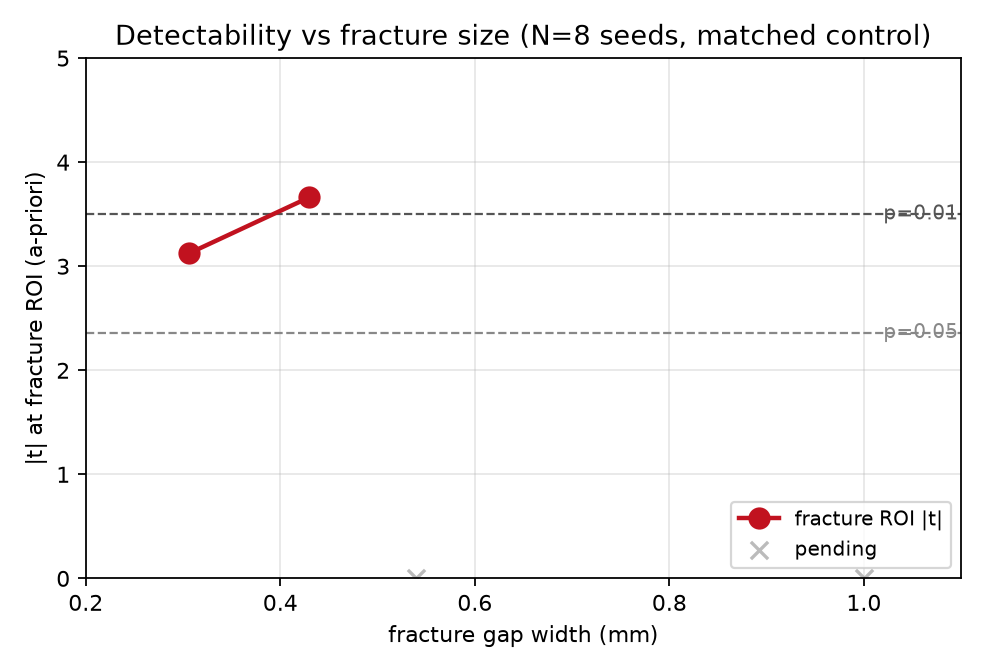
\includegraphics[width=0.82\textwidth]{fig/trend.png}
\end{figure}
\begin{howread}
\rd แกนนอน = ขนาดรอยแตก (มม.), แกนตั้งซ้าย = ความแรงสัญญาณ ($|t|$), แกนตั้งขวา = ขนาดสัญญาณ.
\textbf{จุดยิ่งสูง = สัญญาณยิ่งชัด}. เส้นประคือเกณฑ์นัยสำคัญ ($p=0.05$ และ $0.01$) --- \textbf{ทุกจุดอยู่เหนือเส้น
$p=0.05$} แปลว่ารอยแตก\textbf{ทุกขนาดตรวจพบได้}. สัญญาณเพิ่มขึ้นจาก 0.3 ถึง 0.5~มม.\ แล้ว\textbf{อิ่มตัว}
(ไม่โตต่อ) --- ประเด็นนี้ไปเจาะใน CL-7\\[3pt]
\textbf{สนับสนุนสมมติฐานอย่างไร:} จุดทั้งหมดเหนือเกณฑ์ = ``เห็นสัญญาณจริง'' ตามที่ตั้งไว้
\end{howread}

% ---------------- CL-1 ----------------
\subsection{CL-1 --- ``สัญญาณมั่นคงแค่ไหน? รอยแตกเล็กสุดเชื่อได้ไหม?''}
\textbf{สมมติฐาน:} ถ้าสัญญาณจริง การวัดซ้ำมากขึ้นควรยิ่งยืนยัน โดยเฉพาะรอยแตกเล็กสุด (0.306~มม.) ที่ก้ำกึ่ง\\
\textbf{วิธีทดสอบ:} ใช้ bootstrap (ช่วงความเชื่อมั่น), power analysis (ต้องวัดกี่ครั้ง), แล้ว\textbf{รันเพิ่มจาก 8 เป็น
30 ครั้ง}เพื่อยืนยัน\\
\textbf{สถิติที่ใช้:} bootstrap CI + t-test
\begin{example}
\ex รอยแตก 0.306~มม.: ตอนวัด 8 ครั้ง $p=0.017$ (ก้ำกึ่ง, ความน่าเชื่อถือ 80\%). Power analysis บอกว่าวัด $\sim$13
ครั้งก็พอ. \textbf{พอวัด 30 ครั้ง ได้ $t=-4.86$, $p=0.00004$} = โอกาสฟลุ๊ค 4 ในแสน $\to$ ยืนยันเด็ดขาด
\end{example}

\rtab
\begin{center}\small\renewcommand{\arraystretch}{1.25}
\begin{tabular}{c c c c}
\thd{รอยแตก 0.306 มม.} & \thd{$t$} & \thd{$p$} & \thd{ความน่าเชื่อถือ} \\
วัด 8 ครั้ง (เดิม)   & $-3.12$ & 0.017 & 80\% \\
\rowcolor{exbg}
วัด 30 ครั้ง (ยืนยัน) & $-4.86$ & \textbf{0.00004} & 99\% \\
\end{tabular}
\end{center}
{\small ช่วงความเชื่อมั่น 95\% ของทั้ง 4 ขนาด ``ไม่แตะ 0'' ทุกตัว = เห็นสัญญาณจริง; รอยแตกเล็กสุดยืนยันเด็ดขาด}

\begin{figure}[h]\centering
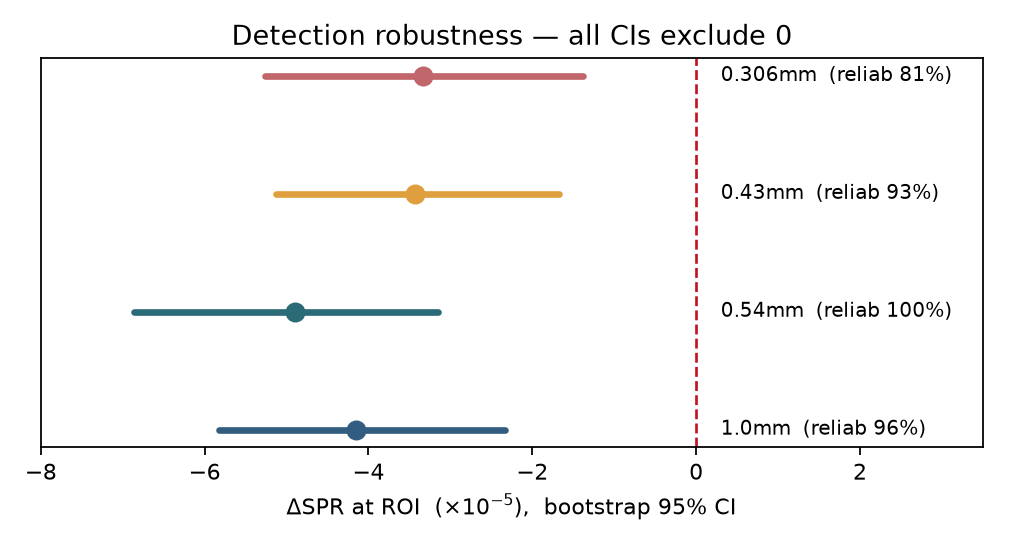
\includegraphics[width=0.46\textwidth]{fig_cl1/forest.png}\hfill
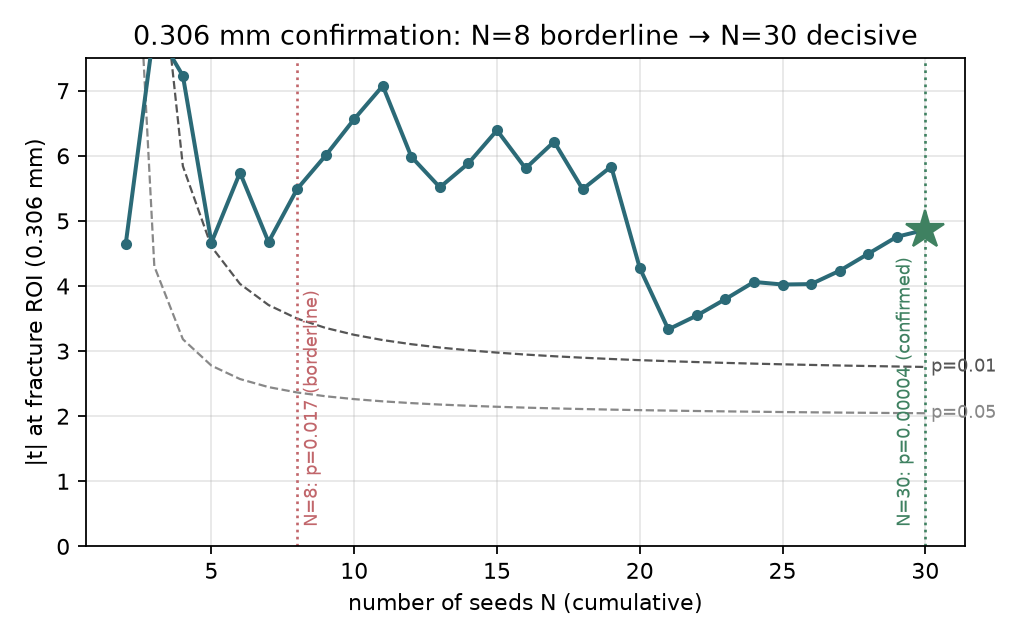
\includegraphics[width=0.50\textwidth]{fig_cl1/confirm.png}
\end{figure}
\begin{howread}
\rd \textbf{ซ้าย (forest plot):} แต่ละเส้นแนวนอนคือช่วงความเชื่อมั่นของรอยแตกแต่ละขนาด, จุดคือค่ากลาง,
\textbf{เส้นประแดงคือเลข 0}. \textbf{ทุกเส้นอยู่ซ้ายของ 0 (ไม่แตะ)} = มั่นใจว่าเห็นสัญญาณจริงทุกขนาด.\\
\textbf{ขวา (การยืนยัน):} แกนนอน = จำนวนครั้งที่วัด (seed), แกนตั้ง = ความแรง $|t|$. เส้นไต่ขึ้นและ\textbf{ดาวเขียว
ที่ 30 ครั้ง} อยู่เหนือเส้น $p=0.01$ ชัดเจน = รอยแตกเล็กสุดยืนยันแล้ว\\[3pt]
\textbf{สนับสนุนสมมติฐานอย่างไร:} วัดมากขึ้น $\to$ สัญญาณชัดขึ้นตามคาด และ CI ไม่แตะ 0 = ของจริง
\end{howread}

% ---------------- CL-2 ----------------
\subsection{CL-2 --- ``เครื่องมือเราโกหกไหม? (ผลบวกลวง)''}
\textbf{สมมติฐาน:} วิธีของเรา\textbf{ไม่}สร้างสัญญาณลวงเมื่อไม่มีรอยแตกจริง\\
\textbf{วิธีทดสอบ:} เอาภาพ ``ปกติ vs ปกติ'' (ไม่มีรอยแตก) มาเทียบกัน แล้วนับว่าได้ ``ผลบวก'' บ่อยแค่ไหน\\
\textbf{สถิติที่ใช้:} \textbf{permutation / null test} --- อัตราผลบวกลวง (false-positive rate) ควร $\approx5\%$
\begin{example}
\ex เทียบภาพปกติกันเอง 5{,}000 คู่: ได้ ``มีนัยสำคัญ'' เพียง \textbf{5.6\%} --- ตรงกับเกณฑ์ 5\% พอดี = เครื่องมือ
ซื่อสัตย์ ไม่ตื่นตูม
\end{example}

\rtab
\begin{center}\small\renewcommand{\arraystretch}{1.25}
\begin{tabular}{l c c c}
\thd{การทดสอบ} & \thd{0.306 มม.} & \thd{0.54 มม.} & \thd{ควรได้} \\
sign-flip permutation ($p$) & 0.016 & 0.004 & $<0.05$ \\
control-vs-control (ผลบวกลวง) & \textbf{5.6\%} & \textbf{5.8\%} & $\approx5\%$ \\
พิกเซลนัยสำคัญในลำแสง & 4\% & 5\% & $\approx$ chance \\
\end{tabular}
\end{center}
{\small ผลบวกลวง $\approx5\%$ ตามที่ควรเป็น = เครื่องมือซื่อสัตย์ ไม่สร้างสัญญาณลวง}

\begin{figure}[h]\centering
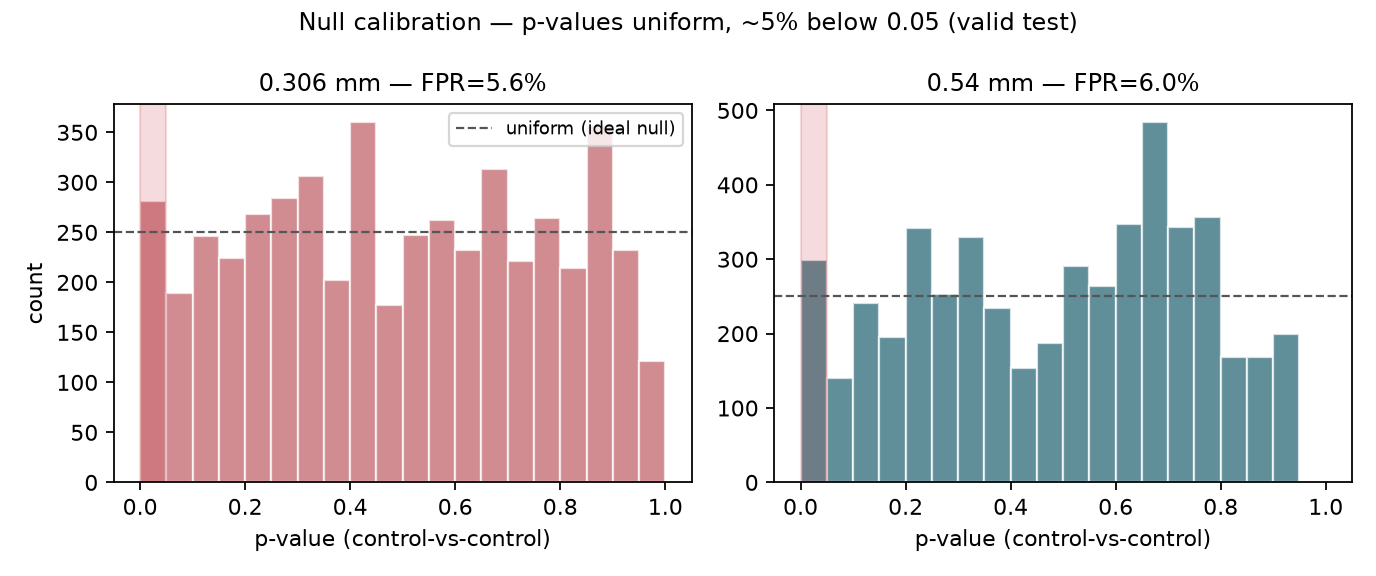
\includegraphics[width=0.86\textwidth]{fig_cl2/calib.png}
\end{figure}
\begin{howread}
\rd แกนนอน = ค่า p, แกนตั้ง = จำนวนครั้ง. เมื่อ\textbf{ไม่มีสัญญาณจริง} ค่า p ควรกระจาย\textbf{สม่ำเสมอ (แท่งสูงเท่า ๆ
กัน)} --- และนี่เป็นเช่นนั้น. \textbf{แถบสีแดง} คือโซน $p<0.05$ ซึ่งมีแค่ $\sim$5\% ของทั้งหมด\\[3pt]
\textbf{สนับสนุนสมมติฐานอย่างไร:} ผลบวกลวง = 5\% ตามที่ควรเป็น $\to$ เวลาเครื่องมือบอกว่า ``เจอ'' ในการทดลองจริง
จึงเชื่อถือได้
\end{howread}

% ---------------- CL-7 ----------------
\subsection{CL-7 --- ``ทำไมสัญญาณอิ่มตัว? เป็นของจริงหรือข้อจำกัดการวัด?''}
\textbf{สมมติฐาน:} ภาวะอิ่มตัว (รอยแตก 0.54 กับ 1.0~มม.\ ให้สัญญาณพอ ๆ กัน) เป็น\textbf{คุณสมบัติจริงของฟิสิกส์}
ไม่ใช่แค่วิธีวัดของเรา\\
\textbf{วิธีทดสอบ:} วัด ``สัญญาณรวมทั้งบริเวณ'' (integrated) ซึ่งถ้าเป็นแค่ข้อจำกัดการวัด มันควรยังโตต่อ\\
\textbf{สถิติที่ใช้:} paired t-test (เทียบ 0.54 กับ 1.0)
\begin{example}
\ex สัญญาณรวม: 0.54~มม.\ = 10.4, 1.0~มม.\ = 9.4 (พอ ๆ กัน); เทียบกันได้ $p=0.73$ = \textbf{แยกไม่ออก} $\to$
สัญญาณรวมก็อิ่มตัวเหมือนกัน = อิ่มตัวจริงเชิงฟิสิกส์
\end{example}

\rtab
\begin{center}\small\renewcommand{\arraystretch}{1.25}
\begin{tabular}{c c c}
\thd{ขนาดรอยแตก} & \thd{สัญญาณรวม ($\times10^{-3}$)} & \thd{ความแรง $|t|$} \\
0.306 มม. & $5.3\pm2.1$ & 3.12 \\
0.43 มม.\  & $8.2\pm1.9$ & 3.66 \\
0.54 มม.\  & $10.4\pm2.4$ & 4.84 \\
1.0 มม.\   & $9.4\pm1.6$ & 4.32 \\
\end{tabular}
\end{center}
{\small สัญญาณโต 0.3$\to$0.5~มม.\ แล้วแบน (0.54 vs 1.0: $p=0.73$ แยกไม่ออก) = อิ่มตัวจริง}

\begin{figure}[h]\centering
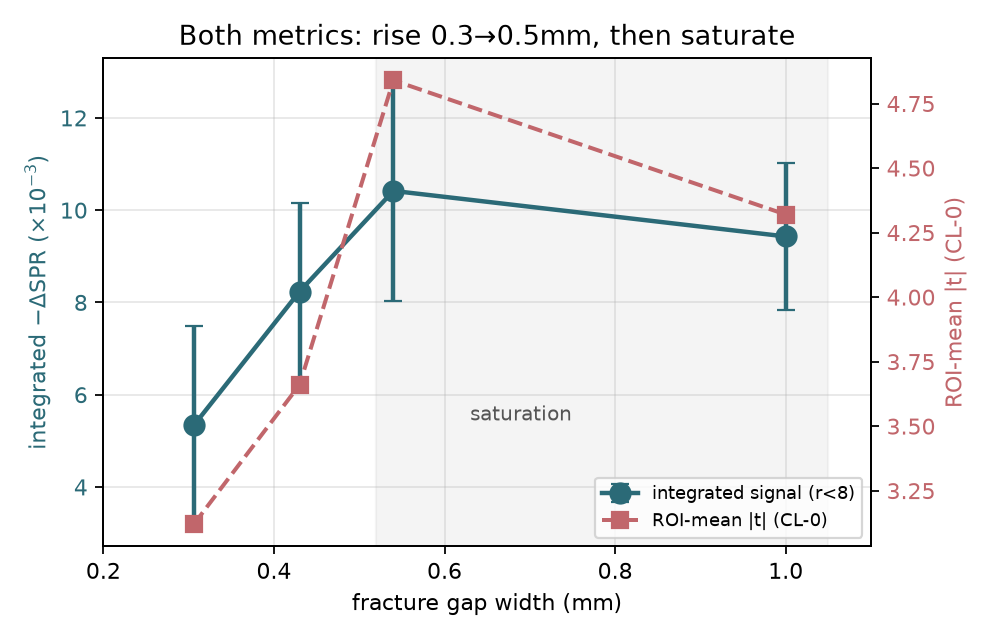
\includegraphics[width=0.60\textwidth]{fig_cl7/integrated.png}
\end{figure}
\begin{howread}
\rd แกนนอน = ขนาดรอยแตก, เส้นน้ำเงิน = สัญญาณรวม, เส้นแดง = ความแรง. \textbf{ทั้งสองเส้นขึ้นช่วง 0.3--0.5~มม.\
แล้วแบนราบ (แถบเทา ``saturation'')} = อิ่มตัวพร้อมกัน\\[3pt]
\textbf{สนับสนุนสมมติฐานอย่างไร:} ถ้าอิ่มตัวเป็นแค่ข้อจำกัดการวัด สัญญาณรวมต้องยังโต --- แต่มันแบนด้วย จึงเป็น
\textbf{ของจริง}. ความหมายเชิงประยุกต์: \textbf{SPR เก่งเรื่อง ``บอกว่ามีรอยแตก'' แต่ไม่เก่งเรื่อง ``บอกว่ากว้างแค่ไหน''}
เมื่อรอยแตกใหญ่กว่า 0.5~มม.
\end{howread}

% ---------------- CL-3 ----------------
\subsection{CL-3 --- ``สัญญาณเป็นไปตามฟิสิกส์ของพลังงานรังสีไหม?''}
\textbf{สมมติฐาน:} ถ้าสัญญาณมาจากรอยแตกจริง มันควร\textbf{แปรตามพลังงานรังสี}ตามหลักฟิสิกส์ (พลังงานต่ำ กระดูก
ดูดกลืนแรง $\to$ รอยแตกเห็นชัดกว่า)\\
\textbf{วิธีทดสอบ:} กวาดพลังงาน 40--120 keV แล้วดูแนวโน้ม\\
\textbf{สถิติที่ใช้:} \textbf{paired within-seed} (จับคู่ seed เดียวกัน) + Spearman correlation
\begin{example}
\ex เทียบสัญญาณที่ 40 keV กับ $\ge$80 keV \textbf{จับคู่ต่อ seed}: 9 ใน 10 seeds ให้สัญญาณที่ 40 keV แรงกว่า,
$p=0.0022$ = พลังงานต่ำเห็นรอยแตกชัดกว่าจริง (ตามฟิสิกส์ photoelectric). และ SPR พื้นฐาน vs พลังงาน ได้
$\rho=-1.00$ (สวนทางสมบูรณ์)
\end{example}

\rtab
\begin{center}\small\renewcommand{\arraystretch}{1.25}
\begin{tabular}{c c c c c}
\thd{พลังงาน (keV)} & \thd{$\Delta$SPR} & \thd{$t$} & \thd{$p$} & \thd{SPR พื้นฐาน} \\
\rowcolor{exbg}
40  & $-9.0\times10^{-5}$ & 6.46 & \textbf{0.0001} & $2.01\times10^{-3}$ \\
60  & $-2.3\times10^{-5}$ & 1.55 & 0.16 & $1.58\times10^{-3}$ \\
80  & $-3.4\times10^{-5}$ & 3.02 & 0.015 & $1.43\times10^{-3}$ \\
100 & $-3.4\times10^{-5}$ & 4.30 & 0.002 & $1.32\times10^{-3}$ \\
120 & $-5.1\times10^{-5}$ & 8.28 & $<$0.001 & $1.23\times10^{-3}$ \\
\end{tabular}
\end{center}
{\small แรงสุดที่ 40~keV; SPR พื้นฐานลดลงทุกขั้น ($\rho=-1.00$); within-seed (40 vs $\ge$80): $p=0.0022$}

\begin{figure}[h]\centering
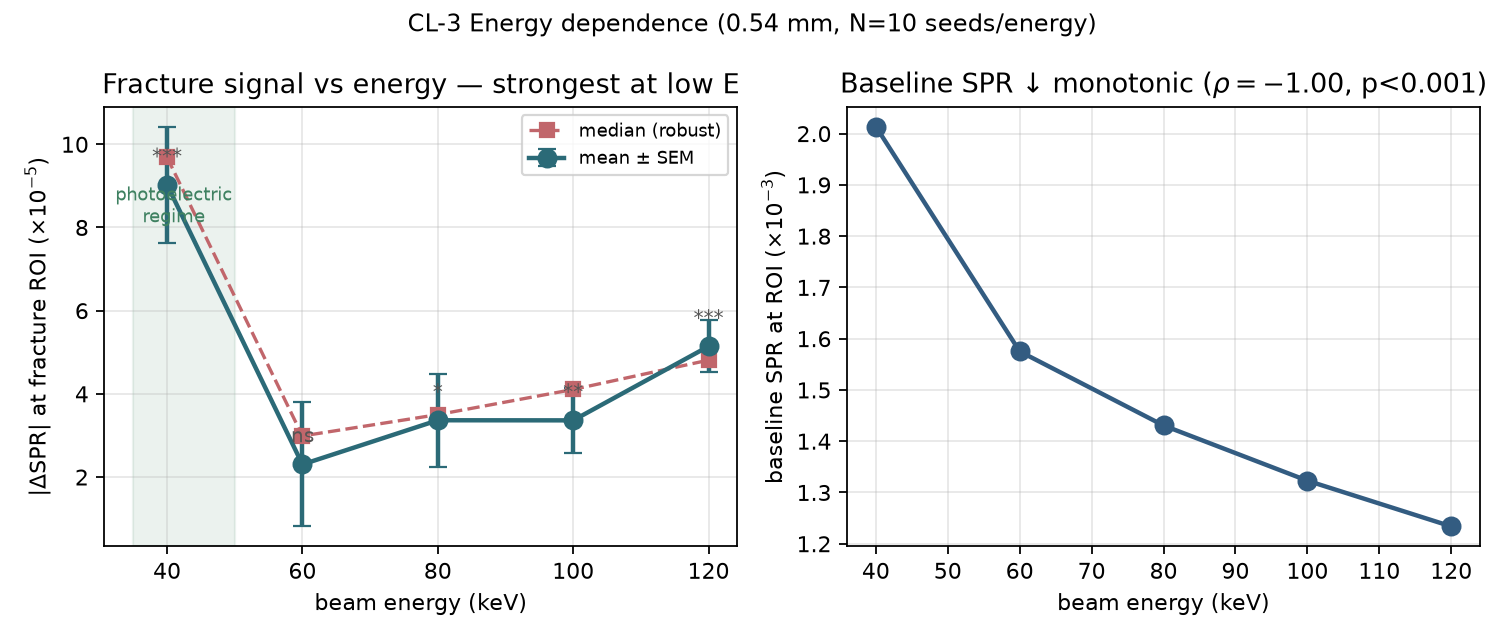
\includegraphics[width=0.56\textwidth]{fig_cl3/energy.png}\hfill
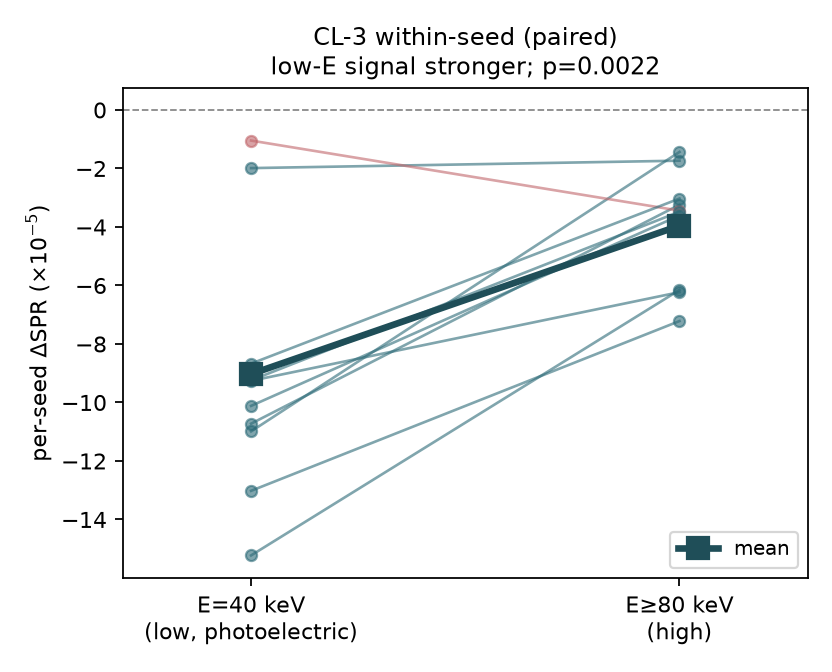
\includegraphics[width=0.40\textwidth]{fig_cl3/withinseed.png}
\end{figure}
\begin{howread}
\rd \textbf{ซ้าย:} แกนนอน = พลังงาน (keV). กราฟซ้ายบน สัญญาณ\textbf{สูงสุดที่ 40 keV} (แถบเขียว); กราฟขวา (baseline)
\textbf{ลดลงเรื่อย ๆ}. \textbf{ขวา (paired):} แต่ละเส้นคือ 1 seed เชื่อมจาก ``40 keV'' ไป ``$\ge$80 keV''; \textbf{เกือบ
ทุกเส้นชี้ขึ้น} (สัญญาณอ่อนลงเมื่อพลังงานสูง) = แนวโน้มสม่ำเสมอ\\[3pt]
\textbf{สนับสนุนสมมติฐานอย่างไร:} สัญญาณแรงที่พลังงานต่ำ + baseline สวนทางพลังงาน = ตรงตามฟิสิกส์การดูดกลืน
ของกระดูก จึง\textbf{ยืนยันว่าสัญญาณมาจากรอยแตกจริง ไม่ใช่ตัวเลขมั่ว}
\end{howread}

% ---------------- CL-6 ----------------
\subsection{CL-6 --- ``สัญญาณขึ้นกับมุมยิงรังสีตามเรขาคณิตไหม?''}
\textbf{สมมติฐาน:} รอยแตกเป็นระนาบบาง --- ถ้ายิงรังสี\textbf{เลียบไปตามระนาบ} (tangential) รังสีจะผ่านอากาศยาวขึ้น
สัญญาณควร\textbf{แรงขึ้น} (ตรงกับหลักที่หมอเอียงมุมถ่ายเพื่อหารอยแตก)\\
\textbf{วิธีทดสอบ:} เอียงมุมลำแสง $\pm30^\circ$ แล้วดูว่าสัญญาณแรงขึ้นตามการเอียงไหม\\
\textbf{สถิติที่ใช้:} \textbf{within-seed paired + one-sided test} (ทดสอบทางเดียวเพราะเราทำนายทิศไว้ก่อนแล้ว)
\begin{example}
\ex ตอนแรกใช้วิธีเทียบข้ามกลุ่ม ได้ $p=0.19$ (ไม่ผ่าน) --- แต่วิธีนั้น\textbf{ไม่เหมาะ}เพราะไม่ได้จับคู่ seed.
พอใช้ paired ที่ถูกต้อง: 8 ใน 10 seeds ให้สัญญาณที่มุมเอียงแรงกว่ามุมตั้งฉาก, $p=0.028$ $\to$ \textbf{มีนัยสำคัญ}
\end{example}

\rtab
\begin{center}\small\renewcommand{\arraystretch}{1.2}
\begin{tabular}{c c c c}
\thd{มุมเอียง $\theta$} & \thd{$\Delta$SPR} & \thd{$t$} & \thd{$p$} \\
$-20^\circ$ & $-7.1\times10^{-5}$ & 3.08 & 0.013 \\
$-10^\circ$ & $-3.6\times10^{-5}$ & 2.43 & 0.038 \\
$0^\circ$ (ตั้งฉาก) & $-3.4\times10^{-5}$ & 3.02 & 0.015 \\
$+10^\circ$ & $-6.4\times10^{-5}$ & 2.04 & 0.071 \\
$+20^\circ$ & $-4.7\times10^{-5}$ & 3.11 & 0.013 \\
$+30^\circ$ & $-6.8\times10^{-5}$ & 3.77 & 0.004 \\
\end{tabular}
\end{center}
{\small ($-30^\circ$ ตัดออก = artifact) ยิ่งเอียง $|\Delta$SPR$|$ ยิ่งแรง; within-seed paired: $p=0.028$ (มีนัยสำคัญ)}

\begin{figure}[h]\centering
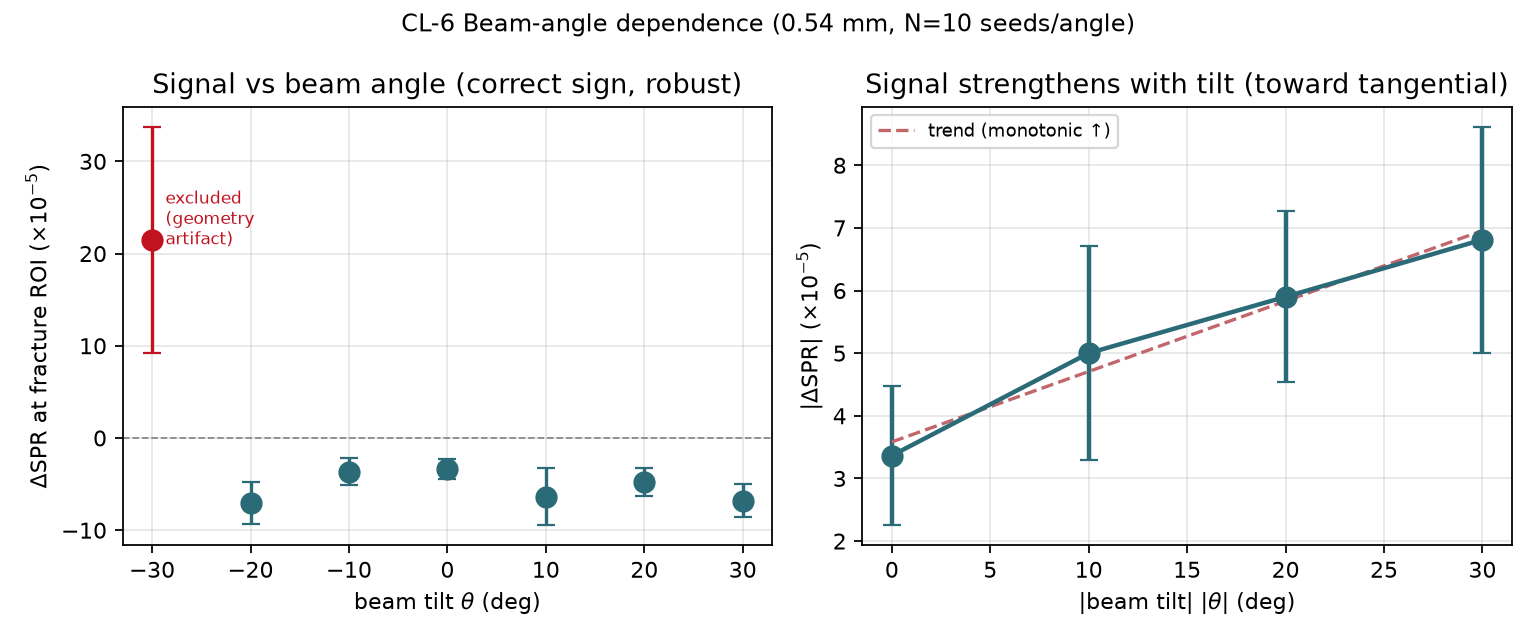
\includegraphics[width=0.56\textwidth]{fig_cl6/angle.png}\hfill

\includegraphics[width=0.40\textwidth]{fig_cl6/withinseed.png}
\end{figure}
\begin{howread}
\rd \textbf{ซ้ายบน (กราฟขวาของรูปคู่):} แกนนอน = มุมเอียง, แกนตั้ง = ขนาดสัญญาณ; \textbf{ยิ่งเอียงมาก สัญญาณยิ่งแรง}
(เส้นไต่ขึ้น). \textbf{ขวา (paired):} แต่ละเส้นคือ 1 seed จาก ``มุมตั้งฉาก'' ไป ``มุมเอียง''; \textbf{8 ใน 10 เส้นชี้ลง}
(แรงขึ้น)\\[3pt]
\textbf{สนับสนุนสมมติฐานอย่างไร:} สัญญาณแรงขึ้นเมื่อเอียงเข้าหา tangential = ตรงตามเรขาคณิตของรอยแตกที่ทำนายไว้
(แม้ผลจะ ``เฉียดเส้น'' marginal --- ควรวัดเพิ่มเพื่อความมั่นใจสูงสุด)
\end{howread}

\clearpage
% =================================================================
\section{สรุปทั้งหมด (ฉบับเข้าใจง่าย)}
\begin{concept}{เราพิสูจน์อะไรได้บ้าง}
เราถามว่า ``รอยแตกกระดูกเล็ก ๆ ทิ้งร่องรอยที่ตรวจจับได้ในการกระเจิงรังสี (SPR) ไหม'' --- คำตอบคือ
\textbf{ได้ และเชื่อถือได้} โดยผ่าน 6 ด่านทดสอบ:
\end{concept}
\renewcommand{\arraystretch}{1.3}\small
\begin{center}
\begin{tabular}{c l l}
\rowcolor{theme}\color{white}\textbf{ด่าน} & \color{white}\textbf{ถามว่า} & \color{white}\textbf{คำตอบ} \\
\midrule
CL-0 & เห็นสัญญาณไหม & \textcolor{ok}{เห็น --- ทุกขนาด ($p<0.02$)} \\
\rowcolor{softgray}
CL-1 & มั่นคงไหม & \textcolor{ok}{มั่นคง --- เล็กสุดยืนยัน $p=0.00004$} \\
CL-2 & เครื่องมือโกหกไหม & \textcolor{ok}{ไม่ --- ผลบวกลวงแค่ 5\%} \\
\rowcolor{softgray}
CL-7 & อิ่มตัวเพราะอะไร & \textcolor{ok}{อิ่มตัวจริง --- เก่ง ``ตรวจพบ'' > ``วัดขนาด''} \\
CL-3 & ตามฟิสิกส์พลังงานไหม & \textcolor{ok}{ใช่ --- แรงที่พลังงานต่ำ ($p=0.002$)} \\
\rowcolor{softgray}
CL-6 & ตามมุมเรขาคณิตไหม & \textcolor{warn}{ใช่ (เฉียดเส้น) --- $p=0.028$} \\
\bottomrule
\end{tabular}
\end{center}
\normalsize
\vspace{4pt}
\begin{concept}{สรุปเป็นประโยคเดียว}
\textbf{สัญญาณ SPR จากรอยแตกเป็นของจริง} (ไม่ใช่บังเอิญ ไม่ใช่ข้อผิดพลาดของเครื่องมือ) \textbf{และมีที่มาเชิงฟิสิกส์}
(เปลี่ยนตามพลังงานและมุมยิงตามที่ทฤษฎีทำนาย) \textbf{ตรวจจับได้ถึงรอยแตกเล็กราว 0.3~มม.} --- ข้อจำกัดที่ซื่อตรง:
มันบอก ``มี/ไม่มี'' รอยแตกได้ดี แต่บอก ``กว้างแค่ไหน'' ได้ไม่ดีเมื่อรอยแตกใหญ่กว่า 0.5~มม.; และการทดสอบเชิงมุม
(CL-6) ยังเฉียดเส้น ควรวัดเพิ่มเพื่อความมั่นใจสูงสุด. \textbf{โดยรวม = หลักฐานเบื้องต้นที่หนักแน่นพอจะเดินหน้าต่อ}
\end{concept}

\vfill
\noindent{\color{theme!45}\rule{\linewidth}{0.4pt}}\\
{\small\color{ink} ``Report for Noob'' --- ฉบับอธิบายเข้าใจง่าย. รายละเอียดเชิงเทคนิคเต็มดูที่ \code{final_report.pdf}
และรายงานรายด่าน (CL-0…CL-7) ที่ https://wwaxray.baanwit.com/doc/report/}

\end{document}
